\documentclass[runningheads]{llncs}
\usepackage[utf8]{inputenc}
\usepackage[english]{babel}
\usepackage[T1]{fontenc}
\usepackage{graphicx}
\usepackage{amsmath}
\usepackage{amssymb}
\usepackage{url}
\usepackage{cite}
\usepackage{tabularx}
\usepackage{rotating}

\title{Learning-Enhanced Security-Constrained\\ Unit Commitment Problem}


\author{Egor Grishin\inst{1}}
\authorrunning{E. Grishin}

\institute{Skoltech, Moscow, Russia}

\begin{document}
\maketitle

\begin{abstract}
The Security-Constrained Unit Commitment (SCUC) problem determines day-ahead generator schedules for power systems while maintaining grid stability. It requires finding minimum-cost generator commitments that satisfy power flow limits and N-1 security criteria. The challenge is that these constraints create large-scale mixed-integer programs, which are computationally intensive due to their combinatorial nature and the need for precise integer solutions, making them difficult for standard solvers to handle efficiently. We combine machine learning with traditional MILP solving to speed up the solution process. In this study we evaluate k-nearest-neighbor warm starts, branching hints, screening of post-contingency constraints, and lazy N-1 enforcement. The aim of this article is to identify combinations of techniques that improve solve time without degrading solution quality. Tests across six MATPOWER cases (14 to 300 buses) show that the dominant gains come from reducing or delaying post-contingency constraints: the best configuration reaches up to 25.8x speedup on case89pegase and 8.6x on average across the six benchmark cases, while warm starts and hints provide smaller secondary gains (around 1.1x). Follow-up runs on case1354pegase confirm that constraint-economy variants remain the most effective at larger scales.
\keywords{Hybrid approach \and Large-scale problem \and Machine learning \and Mixed-integer linear programming \and Unit commitment.}
\end{abstract}


\section{Introduction}
We tackle the Security-Constrained Unit Commitment (SCUC) problem, determining which generators run at what capacity over a 24-hour horizon while keeping costs low and the grid stable. SCUC sits at the core of day-ahead electricity markets, where solutions must be found quickly and reliably.

The computational difficulties come from two sources. First, thermal generators have minimum runtime requirements and cannot change output arbitrarily fast between hours. These temporal constraints tie decisions across all time periods, preventing simple hour-by-hour optimization. Second, we enforce N-1 security: the grid must survive any single component failure (transmission line or generator). For each hour, hundreds or thousands of contingency scenarios must be checked explicitly. With transmission lines numbering in the hundreds, these constraints grow quadratically, creating computational bottlenecks for real-world grids.

Standard MILP solvers cannot handle this scale efficiently. Adding renewable energy's variability makes the problem worse. Even state-of-the-art algorithms hit time limits before finding even suboptimal solutions for large grids, a critical issue when markets clear on strict schedules. We need acceleration methods that maintain solution quality while significantly reducing solve time.

The formulations for the SCUC problem have evolved significantly, transitioning from early heuristics~\cite{Merlin1983} to the more sophisticated and computationally efficient modern MILP models. A computationally efficient MILP formulation for thermal unit commitment with piecewise-linear costs was introduced in~\cite{Carrion2006}. More accurate formulations for complex unit dynamics have since been developed~\cite{Ostrowski2012}. Decomposition methods such as Benders' decomposition and Lagrangian relaxation are often used to separate the main commitment problem from the power grid and security subproblems~\cite{Morales2013, Pan2016}.


On the power grid modeling side, the DC power flow approximation is the standard for SCUC due to its linearity and scalability. Power Transfer Distribution Factors (PTDFs) are widely used to model base-case flows, while Line Outage Distribution Factors (LODFs) provide an efficient way to approximate post-contingency flows without solving the power flow problem for each contingency~\cite{Christie2000, Tejada2018}.

To manage the quadratic growth of contingency constraints, a dynamic constraint generation technique is often adopted~\cite{Tejada2018}.
In this approach, a subset of potential binding constraints is initially included, and additional constraints can be added as necessary during the branching process~\cite{Tejada2018}. A complementary approach involves screening techniques that aim to discard redundant contingencies in advance using power grid sensitivities or historical data~\cite{Holzer2024}.

Machine learning offers a transformative path forward \cite{Bengio2021}, fundamentally altering the approach to solving the SCUC problem by enabling predictive analytics for commitment schedules~\cite{Xavier2019, Quarm2021}, proactive constraint management~\cite{Donti2021}, and the generation of high-quality initial solutions for MILP solvers~\cite{JimenezCordero2022}. For context, Xavier~\textit{et al.}~\cite{Xavier2019} report up to $4.3\times$ speedup on a 6515-bus system using learned active-set predictors, and Jim{\'e}nez-Cordero \textit{et al.}~\cite{JimenezCordero2022} report roughly $2$--$10\times$ on MIPLIB-style instances for warm-starting constraint generation. Our best average speedup is in the same order of magnitude but is obtained with a substantially simpler learning pipeline (1-NN screening plus lazy LODF-based enforcement) that preserves exact N-1 feasibility by construction. Wrong ML predictions, on the other hand, risk grid reliability: a bad warm start or a missed contingency constraint could translate into blackouts, which motivates our decision to apply machine learning only inside an exact MILP framework.

Our solution is in usage of ML acceleration inside an exact MILP framework. The ML components speed things up, while the MILP guarantees correctness. We test multiple ML techniques - warm starts, branching guidance, constraint screening - both individually and combined, identifying which configurations work best. The electrical grid is modeled using the DC approximation, chosen for its balance of accuracy and computational efficiency. In this model, base-case flows are calculated using Power Transfer Distribution Factors (PTDF), and the impacts of line outages are modeled with Line Outage Distribution Factors (LODF), allowing for a linear and scalable representation of grid dynamics crucial for solving the SCUC problem.

\section{Model Definition}

A deterministic SCUC problem is solved over a discrete set of time periods $\mathcal{T}=\{0,\dots,T-1\}$. The power system contains a set of thermal generating units $\mathcal{G}$, buses $\mathcal{B}$, transmission lines $\mathcal{L}$, and reserve products $\mathcal{R}$.

The primary decision variables are defined for each thermal generator $g\in\mathcal{G}$ and time period $t\in\mathcal{T}$ as follows:
\begin{itemize}
    \item Commitment status $u_{g,t}\in\{0,1\}$, which indicates if the generator is on ($1$) or off ($0$).
    \item Startup and shutdown indicators $v_{g,t}, w_{g,t}\in\{0,1\}$, which indicate a change in commitment status.
    \item Segmented power output $p^{\mathrm{seg}}_{g,t,s}\ge 0$, representing the power produced in each segment $s \in \mathcal{K}_g$ of the generator's piecewise-linear cost curve, where $\mathcal{K}_g$ is set of corresponding segments for generator $g$.
    \item Total generation $p_{g,t}$, defined as $p_{g,t}=u_{g,t}\underline{P}_{g,t}+\sum_{s}p^{\mathrm{seg}}_{g,t,s}$, where $\underline{P}_{g,t}$ is the minimum stable generation level.
    \item Reserve provision $r_{k,g,t}\ge 0$ for each reserve product $k\in\mathcal{R}$.
    \item System-wide reserve shortfall $h_{k,t}\ge 0$ for each reserve product $k\in\mathcal{R}$.
\end{itemize}

For the transmission grid, the variables for each line $\ell\in\mathcal{L}$ and time $t\in\mathcal{T}$ are:
\begin{itemize}
    \item Base-case power flow $f_{\ell,t}\in\mathbb{R}$.
    \item Base-case overflow slack variables $\overline{o}_{\ell,t},\underline{o}_{\ell,t}\ge 0$.
    \item Shared N-1 contingency overflow slack variables $\overline{c}_{\ell,t},\underline{c}_{\ell,t}\ge 0$.
\end{itemize}

The operational logic for thermal units is enforced through a set of inter-temporal constraints. The power produced in each segment is constrained by the unit's commitment status and segment capacity, $A_{g,s,t}$:
\begin{equation}
0\le p^{\mathrm{seg}}_{g,t,s} \le A_{g,s,t}\,u_{g,t}, \ \forall g,t,s. \label{eq:seg-link}
\end{equation}
The system-wide power balance must be maintained at each time period, with total generation equal to total demand, $D_{b,t}$:
\begin{equation}
\sum_{g}\Big(u_{g,t}\underline{P}_{g,t}+\sum_{s\in \mathcal{K}_g}p^{\mathrm{seg}}_{g,t,s}\Big)=\sum_{b}D_{b,t}, \ \forall t. \label{eq:balance}
\end{equation}
The availability of reserves is limited by the capacity between the current operating point of a unit and its maximum output, $\overline{P}_{g,t}$:
\begin{equation}
\sum_{s\in \mathcal{K}_g}p^{\mathrm{seg}}_{g,t,s}+\sum_{k}r_{k,g,t}\le (\overline{P}_{g,t}-\underline{P}_{g,t})u_{g,t}, \ \forall g,t. \label{eq:res-head}
\end{equation}
The total reserve provided must be equal to the system requirement $R_{k,t}$ minus penalized shortfall:
\begin{equation}
\sum_{g}r_{k,g,t} + h_{k,t} \ge R_{k,t}, \ \forall k,t. \label{eq:res-req}
\end{equation}
Logical constraints define the startup and shutdown events based on changes in commitment status:
\begin{align}
u_{g,t}-u_{g,t-1} &= v_{g,t}-w_{g,t}, \label{eq:su-def}\\
v_{g,t}+w_{g,t} &\le 1. \label{eq:su-excl}
\end{align}
Ramping constraints limit the rate of change of power output between periods based on ramp-up ($RU_g$), ramp-down ($RD_g$), startup ($SU_g$), and shutdown ($SD_g$) limits:
\begin{align}
p_{g,t}-p_{g,t-1} &\le RU_g\,u_{g,t-1} + SU_g\,v_{g,t}, \label{eq:ramp-up}\\
p_{g,t-1}-p_{g,t} &\le RD_g\,u_{g,t} + SD_g\,w_{g,t}. \label{eq:ramp-dn}
\end{align}
Minimum up-time ($U_g$) and down-time ($D_g$) requirements are enforced:
\begin{align}
\sum_{\tau=t-U_g+1}^{t} v_{g,\tau} \le u_{g,t}, \quad
\sum_{\tau=t-D_g+1}^{t} w_{g,\tau} \le 1-u_{g,t}. \label{eq:min-ud}
\end{align}

The DC power flow model provides a linear approximation of grid physics. Net power injection at each bus is defined:

\begin{equation}
\mathrm{inj}_{b,t}=\sum_{g\in\mathcal{G}_b} p_{g,t} - D_{b,t},
\end{equation}
where $\mathcal{G}_b \subseteq \mathcal{G}$ is the set of generators connected to bus $b$.

The base-case flow on each line $\ell$ is then calculated as a linear combination of these injections, weighted by the pre-computed PTDFs:
\begin{equation}
f_{\ell,t}=\sum_{b\neq b^{\mathrm{ref}}}\mathrm{PTDF}_{\ell,b}\,\mathrm{inj}_{b,t},
\label{eq:flow-def}
\end{equation}
where $b^{\mathrm{ref}}$ is the reference bus.

These flows must respect the line's normal thermal rating, $F^{\mathrm{N}}_{\ell,t}$. With non-negative slack variables $\overline{o}_{\ell,t},\underline{o}_{\ell,t}$, the two-sided bound
\begin{equation}
-F^{\mathrm{N}}_{\ell,t}-\underline{o}_{\ell,t} \ \le\ f_{\ell,t}\ \le\ F^{\mathrm{N}}_{\ell,t}+\overline{o}_{\ell,t}
\label{eq:base-lims}
\end{equation}
is imposed on each line, which is equivalent to the pair of linear inequalities $f_{\ell,t}\le F^{\mathrm{N}}_{\ell,t}+\overline{o}_{\ell,t}$ and $-f_{\ell,t}\le F^{\mathrm{N}}_{\ell,t}+\underline{o}_{\ell,t}$.
To ensure N-1 security, the post-contingency flow on a monitored line $\ell$ following the outage of a line $m$ is approximated using the LODF:
\begin{equation}
f_{\ell,t}^{m} \approx f_{\ell,t}+\mathrm{LODF}_{\ell,m}f_{m,t}. \label{eq:lodf}
\end{equation}
These post-contingency flows must remain within a higher emergency rating, $F^{\mathrm{E}}_{\ell,t}$. A single pair of shared slack variables per monitored line captures the worst-case violation across all contingencies:
\begin{equation}
-F^{\mathrm{E}}_{\ell,t}-\underline{c}_{\ell,t}\ \le\ f_{\ell,t}+\mathrm{LODF}_{\ell,m}f_{m,t}\ \le\ F^{\mathrm{E}}_{\ell,t}+\overline{c}_{\ell,t}.
\label{eq:cont-line}
\end{equation}
For generator outages, if generator $g$ is connected to bus $b(g)$, the post-contingency flow is approximated with the PTDF coefficient of that bus and bounded symmetrically:
\begin{equation}
-F^{\mathrm{E}}_{\ell,t}-\underline{c}_{\ell,t}\ \le\ f_{\ell,t}-\mathrm{PTDF}_{\ell,b(g)}\,p_{g,t}\ \le\ F^{\mathrm{E}}_{\ell,t}+\overline{c}_{\ell,t}.
\label{eq:cont-gen}
\end{equation}


The objective function minimizes total system operating cost, including production costs, startup costs, and penalties for constraint violations:

\begin{align}
\min \ \ & \sum_{t}\sum_{g}\Big( C^{\min}_{g,t}\,u_{g,t} + \sum_{s\in\mathcal{K}_g} C^{\mathrm{seg}}_{g,s,t}\, p^{\mathrm{seg}}_{g,t,s} \Big) \nonumber\\
& + \sum_{t}\sum_{g} C^{\mathrm{su}}_g\, v_{g,t} \label{eq:obj}\\
& + \sum_{t}\sum_{k\in\mathcal{R}} \pi^{\mathrm{res}}_k\, h_{k,t} \nonumber\\
& + \sum_{t}\sum_{\ell\in\mathcal{L}} \pi^{\mathrm{flow}}_{\ell,t}(\overline{o}_{\ell,t}+\underline{o}_{\ell,t}) \nonumber\\
& + \gamma \sum_{t}\sum_{\ell\in\mathcal{L}} \pi^{\mathrm{flow}}_{\ell,t}(\overline{c}_{\ell,t}+\underline{c}_{\ell,t}). \nonumber
\end{align}
The terms in \eqref{eq:obj} are defined as follows. The first line represents production costs, where $C^{\min}_{g,t}$ is the no-load cost and $C^{\mathrm{seg}}_{g,s,t}$ is the marginal cost for energy in each segment. The second term accounts for startup costs, $C^{\mathrm{su}}_g$. The remaining terms are high-cost penalties for violating soft constraints: $\pi^{\mathrm{res}}_k$ penalizes shortfalls in reserve requirements, while $\pi^{\mathrm{flow}}_{\ell,t}$ penalizes base-case and post-contingency transmission overflows. The multiplier $\gamma>1$ is used to prioritize resolving contingency violations.

\section{Acceleration Framework}
Several acceleration methods are evaluated to enhance the computational performance of the MILP solver. Each technique is assigned a concise label for clear identification during the presentation of computational results. These methods encompass constraint screening, lazy constraint enforcement, warm-starting, and branching guidance.

\paragraph{Constraint Screening (PRUNE-$\tau$)}
To manage the prohibitively large number of post-contingency transmission constraints, screening methods are applied to reduce the set of active constraints. The lightweight screening approach, PRUNE-$\tau$, is based on a 1-nearest-neighbor (1-NN) algorithm. Each problem instance is characterized by a load-profile feature vector that combines the z-scored load series with level-sensitive summary statistics. The z-score for a load series $\{L_t\}_{t=0}^{T-1}$ is calculated as:
\begin{equation}
z_t=\frac{L_t-\mu_L}{\sigma_L}, \ \mu_L=\frac{1}{T}\sum_t L_t, \ \sigma_L^2=\frac{1}{T-1}\sum_t(L_t-\mu_L)^2.
\end{equation}
The final feature vector is
\begin{equation}
\phi=\big[z_0,\dots,z_{T-1},\ \mu_L,\ \max_t L_t,\ \sum_t L_t,\ \sigma_L\big].
\end{equation}
This augmented representation avoids the degenerate case in which two load trajectories differ only by a uniform shift and would otherwise appear identical under pure z-scoring. For a new instance with feature vector $\phi$, its Euclidean distance to each instance $\phi^{(i)}$ in a database of solved cases is computed, $d(i)=\big\|\phi-\phi^{(i)}\big\|_2$. The solution from the nearest neighbor, $\hat{\imath}=\arg\min_i d(i)$, is then used to estimate post-contingency flows for the target scenario. The neighbor index $\hat{\imath}$ provides a full solved dispatch profile. We reuse its generator outputs
$p^{(\hat{\imath})}_{g,t}$ as a prediction for the target instance,
\begin{equation}
p^{\mathrm{pred}}_{g,t} := p^{(\hat{\imath})}_{g,t},
\end{equation}
and combine it with the target demand $D_{b,t}$ to form predicted net injections at each bus:
\begin{equation}
\mathrm{inj}^{\mathrm{pred}}_{b,t}=\sum_{g\in\mathcal{G}_b} p^{\mathrm{pred}}_{g,t} - D_{b,t}.
\end{equation}

This allows for the calculation of the minimum relative emergency margin $s^{m}_{\ell}$ (by calculating flows $f_{\ell,t}$, $f_{m,t}$ using \eqref{eq:flow-def}, \eqref{eq:lodf}), for each monitored line $\ell$ and contingency $m$ across all time periods $t$:
\begin{equation}
s^{m}_{\ell}=\min_t \frac{F^{\mathrm{E}}_{\ell,t}-|f_{\ell,t}+\mathrm{LODF}_{\ell,m}f_{m,t}|}{F^{\mathrm{E}}_{\ell,t}}.
\end{equation}
Contingency-line pairs where $s_{\ell}^m \ge \tau$ are pruned from the model for all time periods. The parameter $\tau$ controls the aggressiveness of the pruning. This 1-NN screener is implemented using SciPy.

\paragraph{Constraint Screening (GNN).}

An alternative screening approach, labeled GNN, employs a Graph Neural Network to score the criticality of each transmission line. The GNN operates on a line graph representation of the power system, where nodes correspond to transmission lines and edges connect lines that share a common bus. Each line-node $\ell=(i,j)$ is described by a feature vector including susceptance, average normal and emergency limits and average endpoint loads.
Supervision is obtained from historical solutions by labeling a line as critical if it is frequently near its
emergency limit:
\begin{equation}
y_\ell= 1\ \iff\ \max_t \frac{|f_{\ell,t}|}{F^E_{\ell,t}} \ge y_{\mathrm{thr}},\ y_{\mathrm{thr}}=0.70.
\end{equation}

A two-layer GraphSAGE classifier with a Binary Cross-Entropy (BCE) loss was trained to predict line criticality probabilities
$\hat p_\ell\in[0,1]$.
At inference, we screen contingency constraints using a fixed threshold $\theta=0.60$:
\begin{align}
\text{line outage } m:\quad &\text{keep }(\ell,m)\iff (\hat p_\ell\ge\theta)\ \text{or}\ (\hat p_m\ge\theta),\\
\text{gen outage } g:\quad  &\text{keep }(\ell,g)\iff \hat p_\ell\ge\theta.
\end{align}
So the line is kept if the post-contingency flow constraint on the monitored line $\ell$ under the outage of line $m$ is associated with at least one line predicted to be critical by the model.

The GNN model is implemented using PyTorch with NetworkX utilized for generating topology features. The GraphSAGE model employs a hidden size of 64 and is trained with the Adam optimizer at a learning rate of $10^{-3}$.
Table~\ref{tab:gnn_ablation} reports the downstream effect of replacing the 1-NN screener with the GNN at different $\tau$ thresholds. Across all thresholds, the GNN retains essentially the same fraction of post-contingency constraints as the 1-NN baseline and produces speedups within $\pm 4\%$ of the 1-NN variant (mean ratio between $0.987$ and $1.035$). We attribute this to the fact that the binding contingencies are dominated by a handful of globally critical corridors that the load-conditioned 1-NN already recovers from the historical binding pattern; the additional structural signal learned by the GNN does not move the retained set enough to change solver runtime. We therefore treat the GNN screener as an exploratory ablation rather than as the recommended default.

\begin{table}[t]\centering
\caption{Ablation of the GraphSAGE screener against the 1-NN baseline. Values are means across the six benchmark cases. ``Kept ratio'' is the fraction of post-contingency constraints retained after screening.}
\label{tab:gnn_ablation}
\small
\begin{tabular}{|l|c|c|c|c|}
\hline
\textbf{Threshold} & \textbf{Speedup (1-NN)} & \textbf{Speedup (GNN)} & \textbf{Ratio} & \textbf{Kept ratio (1-NN / GNN)} \\
\hline
PRUNE-0.10 & 9.64x & 9.58x & 0.987 & 0.05\% / 0.05\% \\
PRUNE-0.20 & 8.68x & 8.63x & 1.004 & 0.12\% / 0.12\% \\
PRUNE-0.30 & 6.96x & 6.90x & 0.997 & 0.47\% / 0.47\% \\
PRUNE-0.50 & 3.56x & 3.61x & 1.018 & 3.00\% / 2.98\% \\
PRUNE-0.80 & 2.39x & 2.42x & 1.035 & 18.12\% / 18.04\% \\
\hline
\end{tabular}
\end{table}


\paragraph{Lazy Enforcement (LAZY, BANDIT)}
Instead of adding all post-contingency security constraints to the initial model, N-1 security is enforced dynamically using a lazy constraint callback within the branching process. This base technique is labeled LAZY. At each incumbent integer-feasible solution $(u,p,f)$ found by the solver, post-contingency flows are calculated for each outage $m$ and each monitored line
$l$ using the line's LODF, denoted $\alpha_{\ell m}$:
\begin{equation}
f^{m}_{\ell,t}=f_{\ell,t}+\alpha_{\ell m} f_{m,t}.
\end{equation}
If any calculated flow $f^{m}_{\ell,t}$ violates its corresponding emergency limit $F^{\mathrm{E}}_{\ell,t}$, one or more linear inequalities of the form~\eqref{eq:cont-line} are generated on demand and added to the MILP model as lazy constraints. This keeps the root LP compact while still guaranteeing that the final solution is N-1 secure. In this study we apply lazy enforcement only to the post-contingency constraints~\eqref{eq:cont-line}--\eqref{eq:cont-gen}, because they are by far the most numerous and their threshold-style slack penalties in the objective weaken the dual bound. The base-case thermal limits~\eqref{eq:base-lims} are retained in the root LP, since they are comparatively few ($|\mathcal{L}|\cdot T$) and their dual impact is bounded; a preliminary experiment in which~\eqref{eq:base-lims} were additionally made lazy did not yield consistent improvement and is therefore not reported here.

A modification to this approach involves adding only the top-$K$ most violated contingencies at each callback, sorting violations by their severity. A more adaptive variant, labeled BANDIT, employs a multi-armed bandit algorithm to dynamically select the parameter $K$ from a finite set of candidate values $\mathcal{K}=\{64,128,256\}$. Each value in $\mathcal{K}$ represents an ``arm'' of the bandit. After a new incumbent is found, the reward is defined as the negative number of lazy constraints added at that callback, $R_t=-N_t^{\mathrm{added}}$, to explicitly prefer smaller LP expansions. The value of $K$ for the subsequent callback, $K_{t+1}$, is selected via an $\varepsilon$-greedy policy with $\varepsilon=0.1$, balancing exploration (random selection) and exploitation (selecting the arm with the best empirical mean reward, $\bar{R}_K$):
\begin{equation}
K_{t+1}=\begin{cases}
\text{uniformly from }\mathcal{K}, & \text{with probability }\varepsilon, \\
\arg\max_{K\in\mathcal{K}}\bar{R}_K, & \text{with probability }1-\varepsilon.
\end{cases}
\end{equation}
These lazy enforcement mechanisms are implemented using the solver's native callback API. As we show in Sec.~\ref{sec:experiments}, the bandit layer brings only a marginal improvement over plain LAZY on the benchmark cases reported here, so we report it primarily as a negative result on adaptive cut-budgeting.


\paragraph{Warm Starts (WARM, GRU)}
To accelerate the discovery of a first feasible solution, the MILP solver is warm-started with initial values derived from machine learning models. A memory-light approach, labeled WARM, uses the 1-NN method described previously to match a new instance with the nearest solved instance in a historical database. The commitment schedules, segment powers, and reserve provisions from the historical solution, denoted as $\big\{u_{g,t},\ p^{\mathrm{seg}}_{g,t,s},\ r_{k,g,t}\big\}_{g,t,s,k}$, are then supplied as the initial values for the corresponding variables in the new problem. To ensure these initial values are solver-friendly, a solver-free repair algorithm is applied. This algorithm enforces minimum up/down times, ramping limits, and generation-load balance through heuristics. For a given commitment schedule $(u_{g,t},v_{g,t},w_{g,t})$ and previous power output $p_{g,t-1}$, the repair routine calculates feasible power bounds at time $t$:
\begin{align}
p^{\mathrm{lb}}_{g,t}&=\max\!\Big\{u_{g,t}\underline{P}_{g,t},\ p_{g,t-1}-\big(RD_g\,u_{g,t}+SD_g\,w_{g,t}\big)\Big\}, \\
p^{\mathrm{ub}}_{g,t}&=\min\!\Big\{u_{g,t}\overline{P}_{g,t},\ p_{g,t-1}+RU_g\,u_{g,t-1}+SU_g\,v_{g,t}\Big\}.
\end{align}
A water-filling algorithm then distributes any residual energy to satisfy the system power balance equation whenever feasible.

A more granular warm-start method, labeled GRU, generates dispatch profiles for each generator using a Gated Recurrent Unit network. A two-layer GRU is trained with Mean Squared Error (MSE) loss to predict the fraction of available reserve capacity used by each generator at each hour. This ``above-minimum'' fraction is defined as:
\begin{equation}
r_{g,t}=\frac{\max\{0,\ p_{g,t}-u_{g,t}\underline{P}_{g,t}\}}{\max\{10^{-6},\,u_{g,t}\big(\overline{P}_{g,t}-\underline{P}_{g,t}\big)\}}\in[0,1].
\end{equation}
At inference, the predicted fraction $\hat r_{g,t}$ determines the above-minimum energy $\hat e_{g,t}=\hat r_{g,t}\big(\overline{P}_{g,t}-\underline{P}_{g,t}\big)$. This energy is then allocated across the generator's power segments proportionally to the segment capacities $A_{g,s,t}$, providing a coherent dispatch trajectory to initialize the power segment variables:
\begin{equation}
\hat p^{\mathrm{seg}}_{g,t,s}=\hat e_{g,t}\,\frac{A_{g,s,t}}{\sum_{s'}A_{g,s',t}}.
\end{equation}
This GRU-based warm start is implemented in PyTorch, with a model architecture featuring a hidden size of 32. In the final benchmark, the GRU initializer was less reliable than the simpler 1-NN warm start on the small and medium cases. We attribute this to two factors. First, MSE-trained fractions $\hat r_{g,t}$ do not preserve ramp or minimum up/down relationships, so the resulting dispatch violates inter-temporal feasibility more often than a direct 1-NN copy of a fully solved historical dispatch and must be rewritten by the repair heuristic. Second, on small cases the solver reaches root feasibility in milliseconds, so the PyTorch inference overhead is no longer negligible relative to the total solve time. We therefore report the GRU initializer as a secondary ablation rather than as a recommended default.


\paragraph{Branching Guidance (HINTS, COMMIT)}
Beyond providing an initial feasible solution, machine learning models can be used to guide the solver's branching decisions. A straightforward technique, labeled HINTS, directly translates the binary commitment values from a warm-start solution into branching hints for the solver. This is achieved by setting the VarHintVal attribute for each commitment variable, with a time-biased branching priority assigned to encourage the solver to explore decisions in early time periods first.


A more sophisticated approach, COMMIT, uses a dedicated classifier to predict commitment probabilities, which inform the solver's search strategy. A Gradient Boosted Decision Tree (GBDT) is trained on historical data to estimate the probability that a generator $g$ is committed at time $t$, $\hat{p}_{g,t}=\Pr[u_{g,t}=1\mid x_{g,t}]$, given a feature vector $x_{g,t}$. The feature set is restricted to inputs available before the solve, including normalized system load, time index, generator capacity limits relative to system scale, ramp and start-up limits, and initial status. At inference, the predicted probabilities are used to configure multiple solver parameters to guide the search:
\begin{align}
\texttt{Start}(u_{g,t})&=\mathbb{I}\{\hat{p}_{g,t}\ge 0.5\}, \\
\texttt{VarHintVal}(u_{g,t})&=\texttt{Start}(u_{g,t}).
\end{align}
This configuration provides an initial guess (Start), a hint value (VarHintVal), and prioritizes branching on variables corresponding to earlier time periods. The GBDT classifier is implemented using CatBoost, configured with 500 iterations, a learning rate of 0.06, and a tree depth of 6.


\section{Computational Experiments}
\label{sec:experiments}

\begin{figure*}
  \centering
  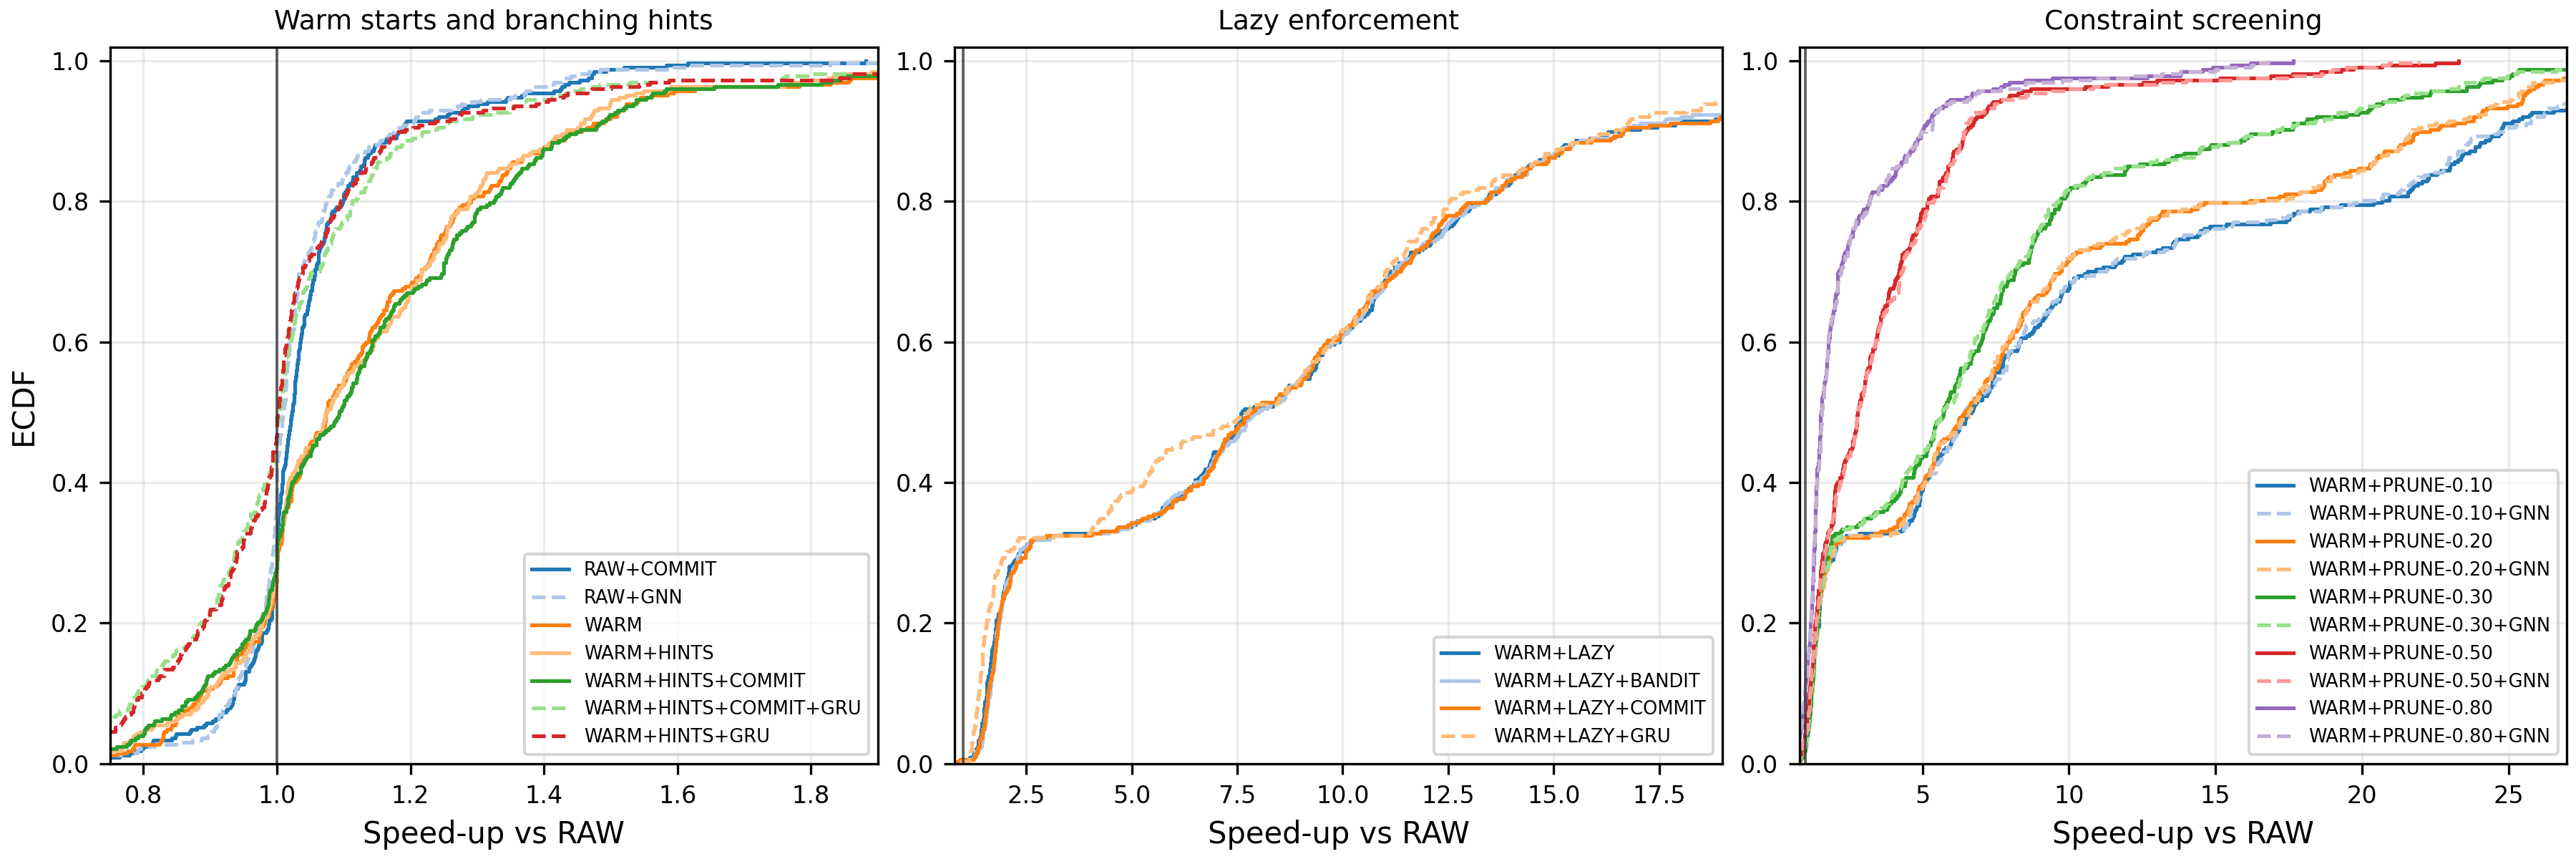
\includegraphics[width=\linewidth]{figures/ecdf.png}
  \caption{Empirical cumulative distribution function of relative speed-up.}
  \label{fig:ecdf}
\end{figure*}

\begin{figure}
  \centering
  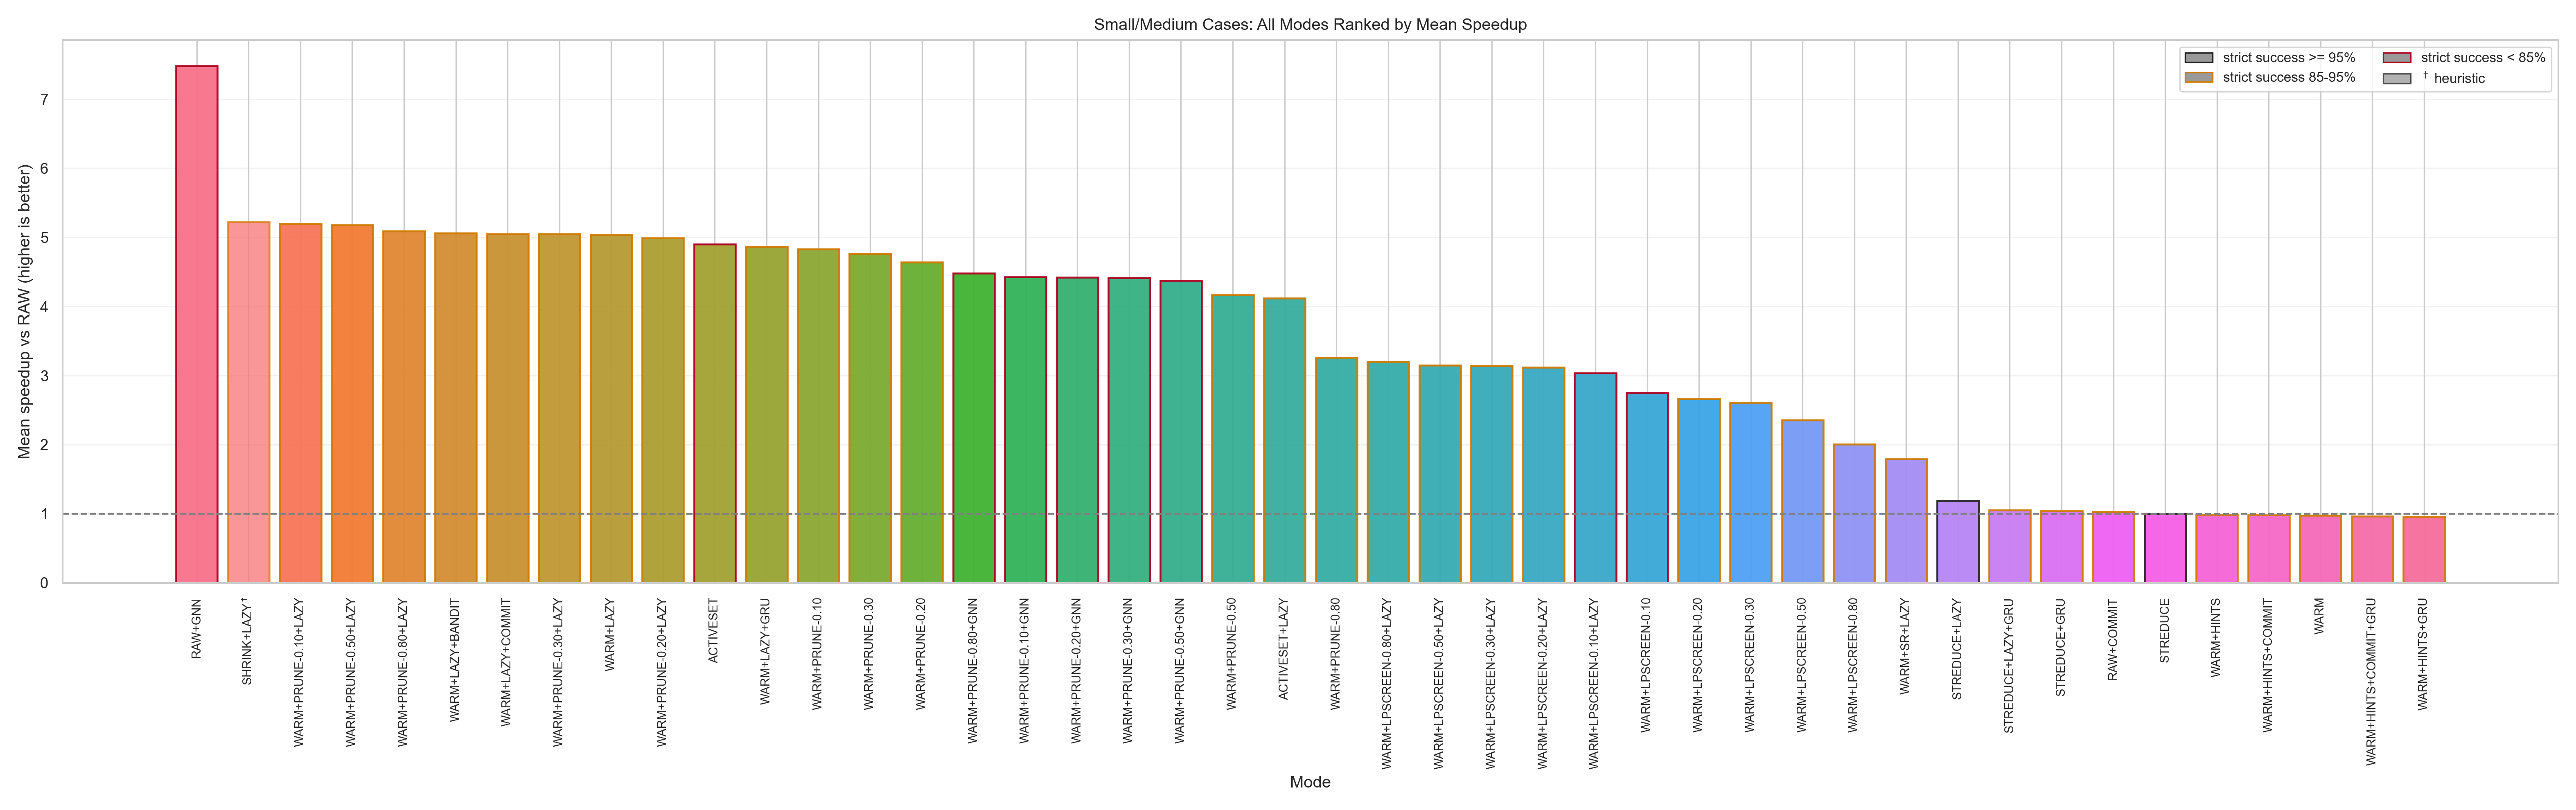
\includegraphics[width=0.8\textwidth]{figures/speedup_general.png}
  \caption{Aggregate speedup distribution across all test cases.}
  \label{fig:Speedup_general}
\end{figure}

All computational experiments were conducted using the Gurobi 12.1 solver on a machine equipped with an AMD Ryzen 7840HS processor and 32 GB of RAM. The benchmark suite consisted of six MATPOWER cases from the UnitCommitment repository~\cite{Xavier2024}, which were used to formulate a multi-period DC-SCUC with full N-1 security constraints (cases 14, 30, 57, 89pegase, 118 and 300). A follow-up evaluation on \texttt{case1354pegase} (1354 buses, 1991 lines) is reported in Sec.~\ref{sec:large}.

For all learning components, the data were split into 70\%/15\%/15\% for training, validation and testing using a fixed random seed. Only the test split was used for all reported results. The speedups were measured relative to a baseline RAW mode, which represented a complete MILP optimization solved without acceleration techniques. Performance was analyzed using the empirical cumulative distribution function (ECDF) of per-instance speedups. In the revision analysis we additionally computed bootstrap 95\% confidence intervals for the main speedup summaries (reported in Tab.~\ref{tab:speedup_ci}) and paired Wilcoxon signed-rank tests against the RAW baseline.


7,702 solver runs were performed across 25 acceleration modes on a final test set of 327 unique problem instances. Total runtime was 73.5 hours. Of these runs, 93.9\% finished with an optimal solution, 4.2\% were infeasible, and 1.9\% terminated due to the time limit.

At the instance level, 95.7\% of the unique instances were solved optimally at least once by one of the tested modes. Smaller cases (14-89 pegase) had a 60-second time limit, while larger cases had a 600-second limit. The training and validation sets were solved over a week.


The robustness of each method is detailed in Tab.~\ref{tab:optimal_cases}. This table reports the percentage of instances solved optimally, found infeasible, or timed out. All variants using lazy enforcement or constraint pruning achieved perfect or near-perfect optimality rates across all test cases.

In contrast, the baseline methods are less robust on larger systems. For example, the RAW+COMMIT variant only solves 71\% of case300 instances optimally within the given time limit, compared to the perfect or near-perfect rates achieved by other methods. For case57, the repeated 77/23/0 pattern is not caused by the acceleration mechanisms: the same 14 dates are reported infeasible by all 23 tested modes, which points to structural infeasibility of those benchmark instances (insufficient reserve after the worst-case contingency) rather than to a screening or warm-start failure. These 14 dates are excluded from the speedup statistics reported below, so they cannot inflate or deflate the reported acceleration factors. In addition, the most aggressive pruning settings can reduce robustness on case300, which indicates that screening must remain conservative if exact feasibility is to be preserved.

Accordingly, the conservative PRUNE-0.10 setting is the recommended screening default in the revised study.

\begin{sidewaystable*}\centering
\caption{Speedup factors with bootstrap 95\% confidence intervals (mean [CI\textsubscript{lo}, CI\textsubscript{hi}]).}
\label{tab:speedup_ci}
\renewcommand{\arraystretch}{1.2}
\footnotesize
\begin{tabular}{|l||c|c|c|c|c|c|}\hline
\textbf{Mode} & \textbf{case14} & \textbf{case30} & \textbf{case57} & \textbf{case89pegase} & \textbf{case118} & \textbf{case300} \\ \hline \hline
RAW+COMMIT & 1.06 [1.02, 1.12] & 1.03 [1.00, 1.07] & 1.06 [1.04, 1.09] & 1.09 [1.05, 1.14] & 1.01 [0.96, 1.04] & 1.02 [0.98, 1.05] \\ \hline
WARM & 1.06 [1.01, 1.12] & 0.98 [0.93, 1.03] & 1.15 [1.11, 1.19] & 1.43 [1.35, 1.52] & 1.03 [1.00, 1.06] & 1.19 [1.12, 1.27] \\ \hline
WARM+HINTS+COMMIT & 1.07 [1.02, 1.13] & 0.95 [0.90, 0.99] & 1.19 [1.15, 1.23] & 1.43 [1.36, 1.52] & 1.02 [0.98, 1.05] & 1.19 [1.12, 1.27] \\ \hline
WARM+LAZY & 1.64 [1.57, 1.74] & 1.85 [1.75, 1.93] & 8.89 [7.51, 10.39] & 12.77 [12.22, 13.34] & 9.04 [8.59, 9.53] & 17.35 [15.38, 19.37] \\ \hline
WARM+LAZY+BANDIT & 1.77 [1.68, 1.87] & 1.83 [1.74, 1.91] & 8.86 [7.53, 10.29] & 12.82 [12.27, 13.41] & 9.03 [8.62, 9.47] & 17.38 [15.39, 19.39] \\ \hline
WARM+PRUNE-0.10 & 1.34 [1.28, 1.42] & 1.41 [1.31, 1.51] & 8.34 [7.05, 9.73] & 25.83 [24.40, 27.26] & 8.22 [7.68, 8.75] & 12.72 [10.95, 14.55] \\ \hline
WARM+PRUNE-0.10+GNN & 1.27 [1.20, 1.34] & 1.42 [1.32, 1.52] & 8.18 [7.04, 9.48] & 25.75 [24.36, 27.14] & 8.17 [7.66, 8.70] & 12.71 [10.96, 14.54] \\ \hline
WARM+PRUNE-0.30 & 1.33 [1.26, 1.40] & 1.41 [1.32, 1.50] & 8.50 [7.19, 9.94] & 16.22 [14.12, 18.30] & 7.37 [6.68, 8.09] & 6.91 [6.11, 7.69] \\ \hline
WARM+PRUNE-0.50 & 1.27 [1.20, 1.34] & 1.44 [1.35, 1.54] & 8.16 [6.91, 9.51] & 3.92 [3.50, 4.40] & 3.08 [2.70, 3.52] & 3.50 [3.15, 3.87] \\ \hline
WARM+PRUNE-0.80 & 1.30 [1.24, 1.35] & 1.45 [1.37, 1.54] & 6.50 [5.60, 7.43] & 2.43 [2.28, 2.59] & 1.05 [0.96, 1.14] & 1.61 [1.49, 1.75] \\ \hline
\end{tabular}
\end{sidewaystable*}


The speedup factors relative to the RAW baseline are summarized in Tab.~\ref{tab:speedup} and Fig.~\ref{fig:Speedup_general}. The best result for each case is highlighted in bold. The strongest average accelerations are delivered by the most conservative screening method and by lazy enforcement. The WARM+PRUNE-0.10 configuration achieves the highest average speedup of 8.56x across the six benchmark cases. Among the lazy enforcement strategies, WARM+LAZY+BANDIT is the strongest variant in this table, attaining an average speedup of 7.47x, although its advantage over plain WARM+LAZY is marginal (mean ratio of per-instance speedups $\approx 1.00$). The results show that the best method can be case-dependent: pruning excels on case89pegase (mean speedup $25.83$x, 95\% CI $[24.40, 27.26]$), while lazy enforcement dominates the largest case in the main benchmark, case300 (mean speedup $17.38$x, 95\% CI $[15.39, 19.39]$). Tab.~\ref{tab:prune_reduction} shows why: on the larger systems, conservative screening eliminates more than 99.7\% of explicit post-contingency constraints before the solve. Conversely, methods that rely only on warm starts and hints without effective constraint management offer little to no acceleration, underscoring that managing the complexity of N-1 security is the primary driver of performance.

The ECDF plot in Fig.~\ref{fig:ecdf}, which contains the most effective methods, illustrates these patterns. PRUNE-0.10 provides consistent gains across the majority of instances. In contrast, the lazy enforcement methods achieve the largest speedups on the most difficult instances, with many runs exceeding a 10x speedup. The paired Wilcoxon tests against RAW confirm that the improvements of WARM+PRUNE-0.10, WARM+LAZY, and WARM+LAZY+BANDIT are statistically significant on every benchmark case ($p<10^{-7}$ in all six cases for each comparison).

These trends are confirmed by the wall-clock runtime statistics in Tab.~\ref{tab:runtime}. For case118, the median time dropped from 43.40 seconds (RAW) to 4.84 seconds with LAZY+BANDIT. For the largest case in the main benchmark, case300, the median runtime improved from 189.90 seconds to just 15 seconds with the same lazy method.
Across several cases, moderately aggressive pruning can solve instances that the RAW baseline fails on within the time limit because the significantly reduced problem size lets the solver explore the search tree more effectively and find a feasible integer solution faster.

\subsection{Large-case follow-up on \texttt{case1354pegase}}
\label{sec:large}

To check that the qualitative picture extends beyond $\le 300$-bus systems, we ran a follow-up evaluation on \texttt{case1354pegase} (1354 buses, 1991 lines). Because the fully explicit N-1 formulation exceeds 9.2M contingency constraints at the root, we restricted the comparison to variants that either keep the contingency set compact by construction (\texttt{SHRINK\_LAZY}, a reduced-topology reformulation) or generate it on demand (\texttt{ACTIVESET\_LAZY}, \texttt{LAZY\_ALL}, \texttt{WARM\_LAZY}). All modes used a 1-hour time limit.
The results in Tab.~\ref{tab:large_case} are consistent with the small-case findings: the compact formulation solves roughly $4\times$ faster than the fully explicit lazy baseline (\texttt{LAZY\_ALL}, median $326$\,s vs $1154$\,s), while warm-start-heavy variants (\texttt{WARM\_LAZY}, \texttt{WARM\_SR\_LAZY}) frequently hit the time limit.
This confirms that on larger systems the dominant bottleneck is still the handling of post-contingency constraints and the quality of the root relaxation, not the absence of branching guidance. We emphasize that \texttt{case1354pegase} (with $\approx 300$ samples per mode still under development) is reported here as a large-scale sanity check rather than as a full statistical evaluation.

\begin{table}[t]\centering
\caption{case300 lazy-runtime sanity check.}
\label{tab:large_case}
\scriptsize
\setlength{\tabcolsep}{2pt}
\resizebox{\linewidth}{!}{%
\begin{tabular}{|l|r|r|r|r|r|r|}
\hline
\textbf{Mode} & \textbf{n} & \textbf{Opt. status} & \textbf{TL} & \textbf{Med. [s]} & \textbf{Root rows} & \textbf{Lazy cuts} \\
\hline
WARM-LAZY & 6 & 100\% & 0\% & 23 & 71,784 & 7,906 \\
SHRINK-LAZY & 6 & 100\% & 0\% & 27 & 15,959 & 0 \\
LAZY-ALL & 6 & 100\% & 0\% & 27 & 71,784 & 8,264 \\
WARM-SR-LAZY & 6 & 100\% & 0\% & 433 & 3,385,032 & 2,212 \\
\hline
\end{tabular}
}
\end{table}


\subsection{Limitations and threats to validity}
\label{sec:limitations}

We list the main limitations of the evaluation so that the claims above can be interpreted correctly.
\begin{itemize}
    \item \emph{Scale.} The benchmark cases (14--300 buses) are smaller than production-scale ISO networks (typically $10^4$--$6\!\cdot\!10^4$ buses). The \texttt{case1354pegase} results in Sec.~\ref{sec:large} are included as a large-scale sanity check, not as a full statistical evaluation.
    \item \emph{Screening reliability.} The 1-NN screener relies on a database of solved instances, whose coverage of operating regimes determines the screening quality. No formal probabilistic guarantee on the fraction of missed binding contingencies is provided; robustness is verified empirically in Tab.~\ref{tab:optimal_cases}.
    \item \emph{Uncertainty.} The formulation is deterministic: renewable variability, load forecasting errors, and stochastic reserve requirements are not modeled.
    \item \emph{Data splits.} Learning components are trained on a single 70\%/15\%/15\% split with a fixed seed. Cross-validation of the resulting speedups is left for future work; the reported Wilcoxon tests concern per-instance differences, not split-level stability.
    \item \emph{Solver tuning.} We compare against the default Gurobi configuration. A systematic comparison with Gurobi's built-in parameter tuning (\texttt{grbtune}) is an important next step, because part of the speedup delivered by our compact formulations may also be achievable via automated tuning.
    \item \emph{Negative results.} The GNN screener (Tab.~\ref{tab:gnn_ablation}), the GRU initializer, and the BANDIT lazy-cut budget are reported here as ablations that did not outperform the simpler baselines; they should be interpreted as negative or inconclusive results in the present benchmark rather than as recommended techniques.
\end{itemize}

\paragraph{Reproducibility.} All ML training pipelines, solver wrappers, and post-processing scripts used to produce the tables and figures in this section will be released as an open-source repository at \url{https://github.com/nemakgregor/SCUCa} together with the benchmark instances and the raw per-instance runtime logs. The main limitations of the evaluation are summarized in Sec.~\ref{sec:limitations}.

\section{Conclusion}

This study demonstrates that, among the methods considered in this work, the most effective way to accelerate a raw mixed-integer linear programming (MILP) formulation of the security-constrained unit commitment (SCUC) problem is to reduce or delay post-contingency constraints while maintaining exact feasibility checks. Across 327 instances of the MATPOWER cases (7702 runs), solved using Gurobi 12.1 on a Ryzen 7840HS/32GB system, two strategies showed the largest and most consistent improvements. The first is screening redundant contingencies prior to solving the model using simple data-driven predictors and LODF/PTDF sensitivities. The second is generating only the necessary contingency constraints on demand during the branching process.

Conservative screening thresholds preserved optimality in all instances, and lazy generation often achieved the best performance on the hardest individual instances. In aggregate, the strongest screening threshold produced the highest average speedup (approximately $8.6\times$ over a fully explicit baseline), while lazy generation dominated the largest case in the main benchmark. The revision analysis also shows that these gains coincide with very large reductions in explicit contingency constraints, typically above 99.7\% on the larger systems, and are statistically significant on every benchmark case (paired Wilcoxon $p<10^{-7}$). The follow-up runs on \texttt{case1354pegase} confirm the same qualitative picture at a much larger scale.

Learning signals applied to the discrete search, including warm starts from historical solutions, lightweight initializers, and branching guidance based on commitment probability, yielded smaller average speedups (around $1.1\times$). In our benchmark, the GNN screener did not consistently outperform the simpler 1-NN baseline, the GRU initializer was unstable on smaller cases, and the adaptive BANDIT policy improved only marginally over plain LAZY. These observations support a ``constraint-economy first'' design: shrink or postpone the contingency set, verify security with exact checks, and only then add inexpensive learning cues to guide the search.

Future work will focus on adapting screening thresholds online, coupling screening with lazy generation in a unified policy, developing reliability-aware predictors with formal guarantees, and benchmarking against Gurobi's built-in automated parameter tuner on the same instances.




\begin{sidewaystable*}\centering
\caption{Optimal case results for all modes (\% optimal / \% infeasible / \% time limit).}
\label{tab:optimal_cases}
\renewcommand{\arraystretch}{1.2}
\footnotesize
\begin{tabular}{|l||c|c|c|c|c|c|c|}\hline\textbf{Mode} & \textbf{case14} & \textbf{case30} & \textbf{case57} & \textbf{case89pegase} & \textbf{case118} & \textbf{case300} \\ \hline \hline
RAW+COMMIT & 100/0/0 & 100/0/0 & 77/23/0 & 100/0/0 & 98/0/2 & 71/0/29 \\ \hline
RAW+GNN & 100/0/0 & 100/0/0 & 77/23/0 & 100/0/0 & 100/0/0 & 71/0/29 \\ \hline
WARM & 100/0/0 & 100/0/0 & 77/23/0 & 100/0/0 & 100/0/0 & 83/0/17 \\ \hline
WARM+HINTS & 100/0/0 & 100/0/0 & 77/23/0 & 100/0/0 & 100/0/0 & 80/0/20 \\ \hline
WARM+HINTS+COMMIT & 100/0/0 & 100/0/0 & 77/23/0 & 100/0/0 & 100/0/0 & 80/0/20 \\ \hline
WARM+HINTS+COMMIT+GRU & 100/0/0 & 100/0/0 & 77/23/0 & 100/0/0 & 100/0/0 & 83/0/17 \\ \hline
WARM+HINTS+GRU & 100/0/0 & 100/0/0 & 77/23/0 & 100/0/0 & 100/0/0 & 83/0/17 \\ \hline
WARM+LAZY & 100/0/0 & 100/0/0 & 77/23/0 & 100/0/0 & 100/0/0 & 100/0/0 \\ \hline
WARM+LAZY+BANDIT & 100/0/0 & 100/0/0 & 77/23/0 & 100/0/0 & 100/0/0 & 100/0/0 \\ \hline
WARM+LAZY+COMMIT & 100/0/0 & 100/0/0 & 77/23/0 & 100/0/0 & 100/0/0 & 100/0/0 \\ \hline
WARM+LAZY+GRU & 100/0/0 & 100/0/0 & 77/23/0 & 100/0/0 & 100/0/0 & 100/0/0 \\ \hline
WARM+PRUNE-0.10 & 100/0/0 & 100/0/0 & 77/23/0 & 100/0/0 & 100/0/0 & 100/0/0 \\ \hline
WARM+PRUNE-0.10+GNN & 100/0/0 & 100/0/0 & 77/23/0 & 100/0/0 & 100/0/0 & 100/0/0 \\ \hline
WARM+PRUNE-0.20 & 100/0/0 & 100/0/0 & 77/23/0 & 100/0/0 & 100/0/0 & 100/0/0 \\ \hline
WARM+PRUNE-0.20+GNN & 100/0/0 & 100/0/0 & 77/23/0 & 100/0/0 & 100/0/0 & 100/0/0 \\ \hline
WARM+PRUNE-0.30 & 100/0/0 & 100/0/0 & 77/23/0 & 100/0/0 & 100/0/0 & 100/0/0 \\ \hline
WARM+PRUNE-0.30+GNN & 100/0/0 & 100/0/0 & 77/23/0 & 100/0/0 & 100/0/0 & 100/0/0 \\ \hline
WARM+PRUNE-0.50 & 100/0/0 & 100/0/0 & 77/23/0 & 100/0/0 & 100/0/0 & 100/0/0 \\ \hline
WARM+PRUNE-0.50+GNN & 100/0/0 & 100/0/0 & 77/23/0 & 100/0/0 & 100/0/0 & 100/0/0 \\ \hline
WARM+PRUNE-0.80 & 100/0/0 & 100/0/0 & 77/23/0 & 100/0/0 & 100/0/0 & 93/0/7 \\ \hline
WARM+PRUNE-0.80+GNN & 100/0/0 & 100/0/0 & 77/23/0 & 100/0/0 & 100/0/0 & 92/0/8 \\ \hline
\end{tabular}
\end{sidewaystable*}

\begin{sidewaystable*}\centering
\caption{Speed-up factors across cases and modes (mean across cases; per-case 95\% CI is reported separately in Tab.~\ref{tab:speedup_ci} for the most important modes).}
\label{tab:speedup}
\renewcommand{\arraystretch}{1.2}
\footnotesize
\begin{tabular}{|l||c|c|c|c|c|c|c|}\hline\textbf{Mode} & \textbf{case14} & \textbf{case30} & \textbf{case57} & \textbf{case89pegase} & \textbf{case118} & \textbf{case300} \\ \hline \hline
RAW+COMMIT & 1.07x & 1.03x & 1.05x & 1.09x & 1.02x & 1.03x \\ \hline
RAW+GNN & 1.05x & 1.02x & 1.03x & 1.09x & 1.01x & 1.02x \\ \hline
WARM & 1.06x & 0.98x & 1.19x & 1.43x & 1.02x & 1.18x \\ \hline
WARM+HINTS & 1.07x & 0.96x & 1.19x & 1.41x & 1.01x & 1.17x \\ \hline
WARM+HINTS+COMMIT & 1.07x & 0.94x & 1.21x & 1.43x & 1.01x & 1.18x \\ \hline
WARM+HINTS+COMMIT+GRU & 0.85x & 0.92x & 1.02x & 1.08x & 1.02x & 1.17x \\ \hline
WARM+HINTS+GRU & 0.87x & 0.93x & 0.99x & 1.07x & 1.01x & 1.16x \\ \hline
WARM+LAZY & 1.65x & \textbf{1.84x} & 6.25x & 12.77x & 8.97x & \textbf{13.14x} \\ \hline
WARM+LAZY+BANDIT & \textbf{1.77x} & 1.84x & \textbf{6.30x} & 12.82x & \textbf{9.00x} & 13.11x \\ \hline
WARM+LAZY+COMMIT & 1.76x & 1.84x & 6.27x & 12.80x & 8.86x & 13.08x \\ \hline
WARM+LAZY+GRU & 1.45x & 1.62x & 5.03x & 12.45x & 8.95x & 13.09x \\ \hline
WARM+PRUNE-0.10 & 1.35x & 1.41x & 5.84x & \textbf{25.83x} & 8.11x & 8.81x \\ \hline
WARM+PRUNE-0.10+GNN & 1.28x & 1.41x & 5.75x & 25.75x & 8.06x & 8.81x \\ \hline
WARM+PRUNE-0.20 & 1.30x & 1.40x & 5.73x & 21.51x & 7.95x & 8.12x \\ \hline
WARM+PRUNE-0.20+GNN & 1.33x & 1.46x & 5.86x & 21.18x & 7.92x & 8.11x \\ \hline
WARM+PRUNE-0.30 & 1.34x & 1.41x & 5.84x & 16.22x & 7.29x & 6.09x \\ \hline
WARM+PRUNE-0.30+GNN & 1.34x & 1.42x & 5.73x & 16.18x & 7.21x & 6.02x \\ \hline
WARM+PRUNE-0.50 & 1.27x & 1.44x & 5.64x & 3.92x & 3.06x & 3.37x \\ \hline
WARM+PRUNE-0.50+GNN & 1.31x & 1.43x & 5.68x & 3.92x & 3.05x & 3.41x \\ \hline
WARM+PRUNE-0.80 & 1.30x & 1.44x & 4.82x & 2.43x & 1.04x & 1.64x \\ \hline
WARM+PRUNE-0.80+GNN & 1.29x & 1.45x & 4.76x & 2.42x & 1.05x & 1.63x \\ \hline
\end{tabular}
\end{sidewaystable*}


\begin{sidewaystable*}
\label{tab:runtime}
\renewcommand{\arraystretch}{1.2}
\footnotesize
\caption{Global runtime statistics (median [min--max])}
\begin{tabular}{|l||c|c|c|c|c|c|c|c|c|}\hline
\textbf{Case} & \textbf{RAW} & \textbf{WARM+LAZY+BANDIT} & \textbf{WARM+PRUNE-0.10} & \textbf{OTHER} \\ \hline \hline
case14 & 0.08 [0.06 - 0.13] & 0.05 [0.03 - 0.07] & 0.06 [0.04 - 0.11] & 0.07 [0.03 - 0.17] \\ \hline
case30 & 0.15 [0.12 - 0.22] & 0.08 [0.06 - 0.17] & 0.11 [0.06 - 0.19] & 0.12 [0.06 - 0.26] \\ \hline
case57 & 0.65 [0.54 - 0.77] & 0.11 [0.08 - 0.20] & 0.12 [0.08 - 0.22] & 0.29 [0.07 - 0.91] \\ \hline
case89pegase & 12.31 [9.19 - 16.84] & 0.97 [0.75 - 1.37] & 0.49 [0.33 - 0.84] & 4.90 [0.35 - 16.24] \\ \hline
case118 & 43.40 [25.79 - 66.25] & 4.84 [3.74 - 7.67] & 5.69 [3.27 - 20.86] & 23.96 [3.12 - 96.22] \\ \hline
case300 & 189.90 [135.81 - 393.03] & 15.00 [11.32 - 20.48] & 22.12 [13.17 - 33.90] & 92.45 [11.26 - 397.51] \\ \hline
\end{tabular}
\end{sidewaystable*}

\begin{table}[t]
\centering
\caption{Average explicit post-contingency constraints retained by WARM+PRUNE-0.10 after screening.}
\label{tab:prune_reduction}
\small
\begin{tabular}{lrrr}
\hline
\textbf{Case} & \textbf{Initial} & \textbf{Retained} & \textbf{Reduction} \\
\hline
case14 & 24,624 & 0 & 100.00\% \\
case30 & 86,112 & 0 & 100.00\% \\
case57 & 441,936 & 0 & 100.00\% \\
case89pegase & 2,459,952 & 504 & 99.98\% \\
case118 & 1,555,992 & 1,026 & 99.94\% \\
case300 & 4,329,720 & 9,109 & 99.79\% \\
\hline
\end{tabular}
\end{table}


\begin{thebibliography}{99}

\bibitem{Merlin1983}
A.~Merlin and P.~Sandrin, ``A new method for unit commitment at Electricit\'e de France,'' \emph{IEEE Trans. Power App. Syst.}, vol.~PAS-102, no.~5, pp.~1218--1225, May 1983.

\bibitem{Carrion2006} M.~Carri\'on and J.~M. Arroyo, ``A computationally efficient mixed-integer linear formulation for the thermal unit commitment problem,'' \emph{IEEE Trans. Power Syst.}, vol.~21, no.~3, pp.~1371--1378, Aug. 2006, doi: 10.1109/TPWRS.2006.876672.

\bibitem{Ostrowski2012}
J.~Ostrowski, M.~F. Anjos, and A.~Vannelli, ``Tight mixed-integer linear programming formulations for the unit commitment problem,'' \emph{IEEE Trans. Power Syst.}, vol.~27, no.~1, pp.~39--46, Feb. 2012.

\bibitem{Morales2013} J.~M. Morales, A.~J. Conejo, H.~Madsen, P.~Pinson, and M.~Zugno, \emph{Integrating Renewables in Electricity Markets: Operational Problems}. New York, NY, USA: Springer, 2013.

\bibitem{Pan2016} K.~Pan and Y.~Guan, ``A polyhedral study of the ramp-up/down constrained unit commitment problem,'' \emph{Math. Program.}, vol.~157, no.~1, pp.~79--113, 2016.

\bibitem{Christie2000}
R.~D. Christie, B.~F. Wollenberg, and I.~Wangensteen, ``Transmission management in the deregulated environment,'' \emph{Proc. IEEE}, vol.~88, no.~2, pp.~170--195, Feb. 2000, doi: 10.1109/5.823997.

\bibitem{Tejada2018} D.~A. Tejada-Arango, P.~S\'anchez-Mart\'in, and A.~Ramos, ``Security constrained unit commitment using line outage distribution factors,'' \emph{IEEE Trans. Power Syst.}, vol.~33, no.~1, pp.~329--337, Jan. 2018.

\bibitem{Holzer2024} J.~T. Holzer, Y.~Chen, Z.~Wu, F.~Pan, and A.~Veeramany, ``Fast simultaneous feasibility test for security constrained unit commitment,'' \emph{IEEE Trans. Power Syst.}, vol.~39, no.~1, pp.~1068--1078, Jan. 2024, doi: 10.1109/TPWRS.2023.3265269.


\bibitem{Bengio2021}
Y.~Bengio, A.~Lodi, and A.~Prouvost, ``Machine learning for combinatorial optimization: A methodological tour d'horizon,'' \emph{Eur. J. Oper. Res.}, vol.~290, no.~2, pp.~405--421, Apr. 2021.

\bibitem{Xavier2019} \'A.~S. Xavier, F.~Qiu, and S.~Ahmed, ``Learning to Solve Large-Scale Security-Constrained Unit Commitment Problems,'' \emph{arXiv preprint} arXiv:1902.01697, 2019. [Online]. Available: \url{https://arxiv.org/abs/1902.01697}

\bibitem{Quarm2021}
E.~Quarm and R.~Madani, ``Scalable security-constrained unit commitment under uncertainty via cone programming relaxation,'' \emph{IEEE Trans. Power Syst.}, vol.~36, no.~5, pp.~4733--4744, Sept. 2021, doi: 10.1109/TPWRS.2021.3062203.

\bibitem{Donti2021} P.~Donti, B.~Amos, Z.~D. Davis, and J.~Z. Kolter, ``DC3: A learning method for optimizing transmission switching in DC optimal power flow,'' \emph{arXiv preprint} arXiv:2104.12225, 2021. [Online]. Available: \url{https://arxiv.org/abs/2104.12225}

\bibitem{JimenezCordero2022}
A.~Jim\'enez-Cordero, J.~M. Morales, and S.~Pineda, ``Warm-starting constraint generation for mixed-integer optimization: A machine learning approach,'' \emph{Knowledge-Based Systems}, vol.~253, p.~109570, Oct. 2022, doi: 10.1016/j.knosys.2022.109570.


\bibitem{Xavier2024}
A.~S. Xavier, A.~M. Kazachkov, O.~Yurdakul, J.~He, and F.~Qiu, ``UnitCommitment.jl (v0.4),'' Zenodo, 2024. [Online]. Available: \url{https://doi.org/10.5281/zenodo.4269874}, \url{https://axavier.org/UnitCommitment.jl/0.4/instances}.

\end{thebibliography}

\end{document}
